% Collatz trajectory of 27: 111 steps, maximum 9232 at step 77.
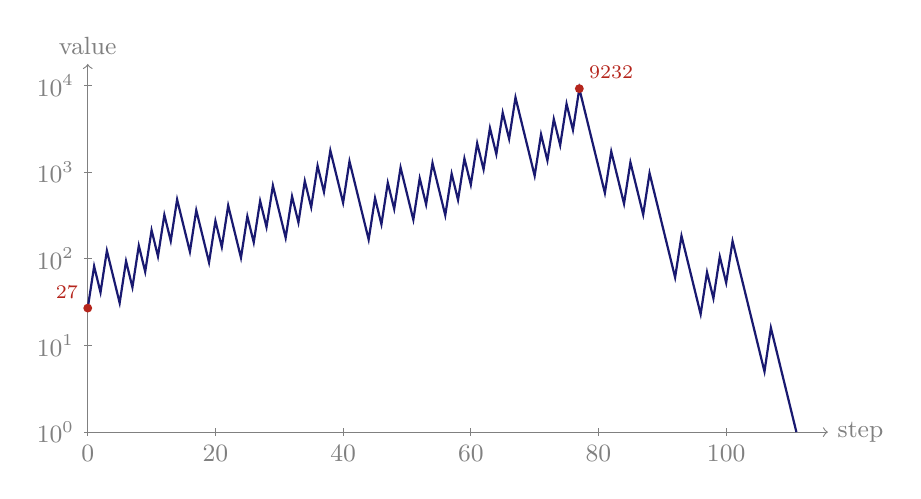
\begin{tikzpicture}[font=\small]
\draw[black!50,->] (0,0) -- (9.4,0) node[right] {step};
\draw[black!50,->] (0,0) -- (0,4.675) node[above] {value};
\draw[black!50] (0.05,0.000) -- (-0.05,0.000) node[left] {$10^{0}$};
\draw[black!50] (0.05,1.100) -- (-0.05,1.100) node[left] {$10^{1}$};
\draw[black!50] (0.05,2.200) -- (-0.05,2.200) node[left] {$10^{2}$};
\draw[black!50] (0.05,3.300) -- (-0.05,3.300) node[left] {$10^{3}$};
\draw[black!50] (0.05,4.400) -- (-0.05,4.400) node[left] {$10^{4}$};
\draw[black!50] (0.000,0.05) -- (0.000,-0.05) node[below] {$0$};
\draw[black!50] (1.622,0.05) -- (1.622,-0.05) node[below] {$20$};
\draw[black!50] (3.243,0.05) -- (3.243,-0.05) node[below] {$40$};
\draw[black!50] (4.865,0.05) -- (4.865,-0.05) node[below] {$60$};
\draw[black!50] (6.486,0.05) -- (6.486,-0.05) node[below] {$80$};
\draw[black!50] (8.108,0.05) -- (8.108,-0.05) node[below] {$100$};
\draw[MidnightBlue,thick] (0.0000,1.5745) -- (0.0811,2.1052) -- (0.1622,1.7741) -- (0.2432,2.3028) -- (0.3243,1.9716) -- (0.4054,1.6405) -- (0.4865,2.1704) -- (0.5676,1.8393) -- (0.6486,2.3675) -- (0.7297,2.0364) -- (0.8108,2.5635) -- (0.8919,2.2323) -- (0.9730,2.7586) -- (1.0541,2.4275) -- (1.1351,2.9533) -- (1.2162,2.6222) -- (1.2973,2.2911) -- (1.3784,2.8172) -- (1.4595,2.4861) -- (1.5405,2.1549) -- (1.6216,2.6815) -- (1.7027,2.3504) -- (1.7838,2.8764) -- (1.8649,2.5453) -- (1.9459,2.2141) -- (2.0270,2.7405) -- (2.1081,2.4094) -- (2.1892,2.9352) -- (2.2703,2.6041) -- (2.3514,3.1296) -- (2.4324,2.7985) -- (2.5135,2.4673) -- (2.5946,2.9931) -- (2.6757,2.6620) -- (2.7568,3.1874) -- (2.8378,2.8563) -- (2.9189,3.3815) -- (3.0000,3.0504) -- (3.0811,3.5755) -- (3.1622,3.2443) -- (3.2432,2.9132) -- (3.3243,3.4384) -- (3.4054,3.1073) -- (3.4865,2.7761) -- (3.5676,2.4450) -- (3.6486,2.9708) -- (3.7297,2.6396) -- (3.8108,3.1651) -- (3.8919,2.8340) -- (3.9730,3.3592) -- (4.0541,3.0281) -- (4.1351,2.6970) -- (4.2162,3.2224) -- (4.2973,2.8912) -- (4.3784,3.4164) -- (4.4595,3.0853) -- (4.5405,2.7542) -- (4.6216,3.2795) -- (4.7027,2.9484) -- (4.7838,3.4735) -- (4.8649,3.1424) -- (4.9459,3.6675) -- (5.0270,3.3363) -- (5.1081,3.8613) -- (5.1892,3.5302) -- (5.2703,4.0551) -- (5.3514,3.7240) -- (5.4324,4.2489) -- (5.5135,3.9177) -- (5.5946,3.5866) -- (5.6757,3.2555) -- (5.7568,3.7805) -- (5.8378,3.4493) -- (5.9189,3.9743) -- (6.0000,3.6432) -- (6.0811,4.1681) -- (6.1622,3.8369) -- (6.2432,4.3618) -- (6.3243,4.0307) -- (6.4054,3.6996) -- (6.4865,3.3684) -- (6.5676,3.0373) -- (6.6486,3.5624) -- (6.7297,3.2313) -- (6.8108,2.9001) -- (6.8919,3.4253) -- (6.9730,3.0942) -- (7.0541,2.7631) -- (7.1351,3.2884) -- (7.2162,2.9573) -- (7.2973,2.6261) -- (7.3784,2.2950) -- (7.4595,1.9639) -- (7.5405,2.4913) -- (7.6216,2.1602) -- (7.7027,1.8290) -- (7.7838,1.4979) -- (7.8649,2.0296) -- (7.9459,1.6985) -- (8.0270,2.2278) -- (8.1081,1.8967) -- (8.1892,2.4245) -- (8.2703,2.0934) -- (8.3514,1.7623) -- (8.4324,1.4311) -- (8.5135,1.1000) -- (8.5946,0.7689) -- (8.6757,1.3245) -- (8.7568,0.9934) -- (8.8378,0.6623) -- (8.9189,0.3311) -- (9.0000,0.0000);
\fill[BrickRed] (6.2432,4.3618) circle (1.6pt) node[above right,font=\scriptsize] {$9232$};
\fill[BrickRed] (0.0000,1.5745) circle (1.6pt) node[above left,font=\scriptsize] {$27$};
\end{tikzpicture}
